\subsection{Analytisches Haar-Wavelet}
\rhead{Analytisches Haar-Wavelet}
Betrachten wir zum Abschluss noch beispielhaft das Haar-Wavelet.
\begin{satz}
    Das dem Haar-Wavelet zugeordnete analytische Wavelet ist
    \[\psi^\ast_{\text{Haar}} = \frac{1}{\sqrt{2}}\left(\psi_{\text{Haar}} + \frac{i}{\pi} \log\left|\frac{t^2-0.5^2)}{t^2}\right|\right).\]
\end{satz}

\begin{proof}
    Die Hilbert-Transformierte des Haar-Wavelets aus Definition~\ref{complex:def-haar} ist
    \begin{align*}
    \mathcal{H} \psi_{\text{Haar}}
    &= \frac{1}{\pi} \CH\int_{-\infty}^{\infty} \frac{\psi_{\text{Haar}}(x)}{t-x} dx\\
    &= \frac{1}{\sqrt2\pi}\left( \CH\int_{-0.5}^{0} \frac{1}{t-x}dx + \CH\int_{0}^{0.5} \frac{-1}{t-x}dx \right)\\
    &= \frac{1}{\sqrt2\pi} \left( -\left[\log \left|t-x\right| \right]_{-0.5}^{0} + \left[\log\left|t-x\right| \right]_{0}^{0.5} \right)\\
    &= \frac{1}{\sqrt2\pi} \left( -\log\left|t\right| + \log\left|t+0.5\right| + \log\left|t-0.5\right| - \log\left|t\right|\right)\\
    &= \frac{1}{\sqrt2\pi} \log\left|\frac{(t+0.5)(t-0.5)}{t^2}\right|
    = \frac{1}{\sqrt2\pi} \log\left|\frac{t^2-0.5^2}{t^2}\right|.
    \end{align*}
    Daraus folgt das zugehörige, analytische Wavelet nach Satz~\ref{complex:analytic-wavelet}.
\end{proof}

Das analytische Haar-Wavelet ist in Abbildung~\ref{complex:ahaar} dargestellt.
Es hat keinen kompakten Träger mehr, ist jedoch noch immer gut lokalisiert in der Zeit.
Abbildung~\ref{complex:ahaar-ex} zeigt die Wavelet-Transformation mit dem analytischen Haar-Wavelet.
Gut ersichtlich sind die scharfe Lokalisierung in der Zeit, die schlecht Lokalisierung in der Frequenz, die Verschiebung zwischen $1/a$ und $f$, so wie die Unabhängigkeit von Amplitude und Phase.

\begin{figure}
	\centering
	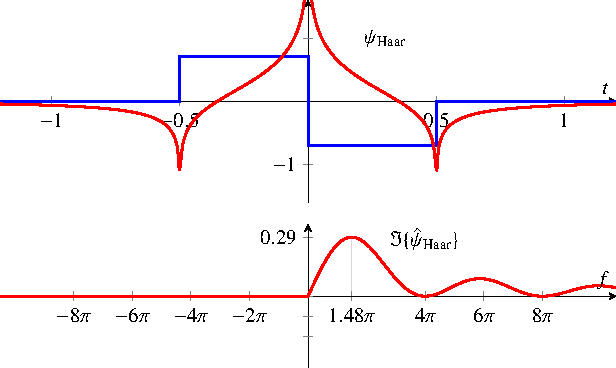
\includegraphics{papers/complex/images/ahaar.pdf}
	\caption{Das analytische Haar-Wavelet im Zeit- und Frequenzbereich.}
	\label{complex:ahaar}
\end{figure}

\begin{figure}
	\centering
	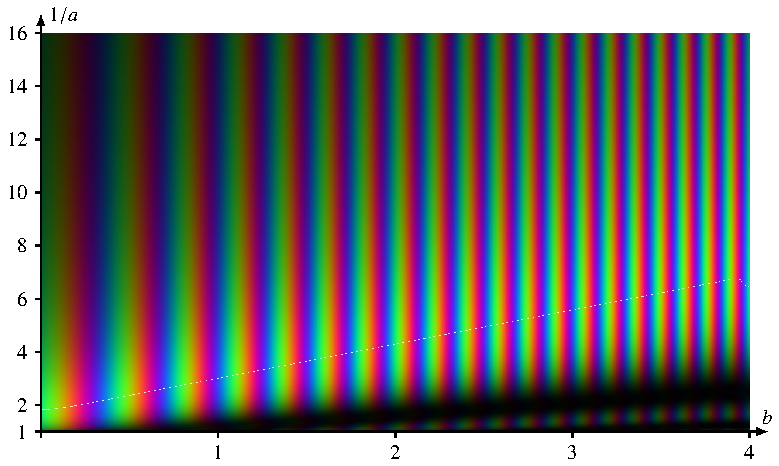
\includegraphics{papers/complex/images/chirp_ahaar.pdf}
	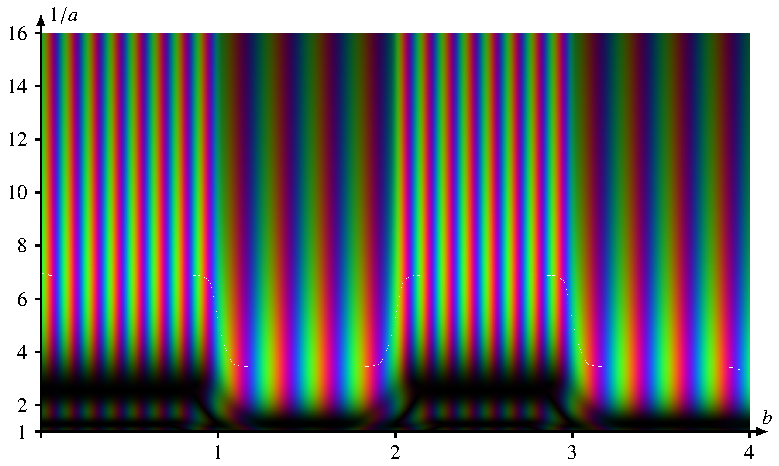
\includegraphics{papers/complex/images/square_ahaar.pdf}
	\caption{Farb-codierte Wavelet-Transformationen der beiden Beispielsignale mit dem \\ analytischen Haar-Wavelet.}
	\label{complex:ahaar-ex}
\end{figure}
